\pdfoutput=1
\documentclass[11pt]{amsart}
\usepackage[T1]{fontenc}
\usepackage[utf8]{inputenc}
\usepackage{lmodern}
\usepackage[margin=1.15in]{geometry}
\usepackage{amsmath,amssymb,amsthm,mathtools}
\usepackage{booktabs}
\usepackage[section]{placeins}
\usepackage{microtype}
\usepackage{enumitem}
\usepackage{xcolor}
\usepackage{tikz}
\usepackage[hidelinks]{hyperref}
\usepackage{xurl}
\usepackage{orcidlink}
\usepackage[capitalise,nameinlink]{cleveref}

\newtheorem{theorem}{Theorem}[section]
\newtheorem{lemma}[theorem]{Lemma}
\newtheorem{corollary}[theorem]{Corollary}
\newtheorem{proposition}[theorem]{Proposition}
\theoremstyle{definition}
\newtheorem{definition}[theorem]{Definition}
\theoremstyle{remark}
\newtheorem{remark}[theorem]{Remark}

\newcommand{\leanus}{\textunderscore\allowbreak}
\newcommand{\lean}[1]{{\ttfamily\let\_\leanus #1}}
\newcommand{\code}[1]{\texttt{#1}}
\newcommand{\fcb}{f_{\mathrm{cubic,bip}}}

\title[Cubic bipartite graphs without cycles of length 4, 8, 16]{Every cubic bipartite graph on at most 84 vertices\\ has a cycle of length 4, 8 or 16}

\author[A. Marszałek]{Andrzej Marszałek\,\orcidlink{0009-0006-6148-2965}}
\address{Independent Researcher}
\urladdr{https://github.com/hipotures/conjectures}

\subjclass[2020]{05C38, 05C35, 05B30, 68V05}
\keywords{Erdős–Gyárfás conjecture, cubic bipartite graphs, symmetric configurations, Levi graphs, exhaustive search, certificates}

\date{27 November 2026}

\begin{document}

\begin{abstract}
The Erdős–Gyárfás conjecture states that every graph of minimum degree at least
three contains a cycle whose length is a power of two. Tranquilli proved that
every cubic bipartite graph on at most $58$ vertices contains a cycle of length
$4$, $8$ or $16$, and Zhuge extended this to $68$ vertices. We extend it to $84$
vertices, so a cubic bipartite counterexample has at least $86$ vertices. The
proof splits into two cases. Graphs with a $6$-cycle are handled by
Tranquilli's triangle-rooted search, which we run with a larger cap. Graphs of
girth at least $10$ are handled by a new search rooted at a forced
$15$-block subtree, which needs no classification of cages and shows that every
cubic bipartite graph of girth at least $10$ on at most $88$ vertices has a
$16$-cycle. Every pruned branch of both searches carries an explicit witness
cycle that a separate checker verifies. The counters agree with Tranquilli's
original program at every cap and with an independent implementation at small
caps. The case split and the soundness of the witness checks are proved in
Lean~4.
\end{abstract}

\maketitle

%======================================================================
\section{Introduction}

\begin{quote}
\textbf{Conjecture} (Erdős and Gyárfás, 1995; see~\cite{Erdos1997}).
Every finite simple graph of minimum degree at least three contains a cycle
whose length is a power of two.
\end{quote}

The conjecture is open. Computer searches exclude small counterexamples:
Ducoffe and Dumitru~\cite{DucoffeDumitru2026} report that a counterexample has
more than $40$ vertices, more than $48$ if it is cubic, and more than $66$ if it
is bipartite. Their computation does not produce proof certificates.

Cubic bipartite graphs are the Levi graphs of symmetric configurations, and
this correspondence makes them well suited to exhaustive search. Tranquilli~\cite{Tranquilli2026}
proved the following stronger statement for $n\le 58$: only the lengths $4$, $8$
and $16$ are needed. Zhuge~\cite{Zhuge2026} extended Tranquilli's search to
$n\le 68$. Both proofs use the fact that a cubic bipartite graph without
$4$- and $8$-cycles on fewer than $70$ vertices has a $6$-cycle (the Moore bound
below $62$ vertices; O'Keefe and Wong's theorem that the smallest cubic graph of
girth $10$ has $70$ vertices~\cite{OKeefeWong1980} for $62\le n\le 68$).

\begin{theorem}\label{thm:main}
Every simple cubic bipartite graph on at most $84$ vertices contains a cycle of
length $4$, $8$ or $16$.
\end{theorem}

\begin{corollary}\label{cor:86}
A cubic bipartite counterexample to the Erdős–Gyárfás conjecture has at least
$86$ vertices.
\end{corollary}

\begin{proof}
A cubic bipartite graph has two colour classes of equal size, so its order is
even; \cref{thm:main} excludes every order up to $84$.
\end{proof}

From $70$ vertices on, girth $10$ is possible, so the reduction to graphs with
a $6$-cycle fails. We handle graphs of girth at least $10$ with a second search
(\cref{sec:branchB}), which gives a statement of independent interest.

\begin{theorem}\label{thm:girth10}
Every simple cubic bipartite graph of girth at least $10$ on at most $88$
vertices contains a $16$-cycle. In particular, the three $(3,10)$-cages contain
a $16$-cycle.
\end{theorem}

\begin{table}[ht]
\centering
\caption{Lower bounds for the order of a cubic bipartite counterexample. The
last two rows require only a cycle of length $4$, $8$ or $16$.}
\label{tab:history}
\begin{tabular}{@{}llll@{}}
\toprule
source & class searched & order excluded & certificates\\
\midrule
Ducoffe--Dumitru~\cite{DucoffeDumitru2026} & bipartite, $\delta\ge 3$ & $n\le 66$ & no\\
Tranquilli~\cite{Tranquilli2026} & cubic bipartite & $n\le 58$ & yes\\
Zhuge~\cite{Zhuge2026} & cubic bipartite & $n\le 68$ & yes\\
this paper & cubic bipartite & $n\le \mathbf{84}$ & yes\\
\bottomrule
\end{tabular}
\end{table}

Let $\fcb(4)$ denote the least order of a cubic bipartite graph without cycles
of length $4$, $8$ and $16$. \Cref{thm:main} gives $\fcb(4)\ge 86$. For
comparison, the least order of a cubic graph without these cycles is
$78$~\cite{Exoo2014,Ripatti2017}, and a graph of minimum degree at least three
without them exists on $73$ vertices~\cite{Marszalek2026}.

\subsection*{Nature of the proof}
The proof is computer-assisted. Its mathematical part, which reduces the
theorem to two finite searches, is short and is written out in
\cref{sec:configs,sec:search}; the case split and the soundness of the witness
checks are also proved in Lean~4 (\cref{sec:lean}). The searches visit about
$2\cdot 10^{10}$ candidate blocks. Each rejection is either a degree or pair
condition that the checker recomputes, or comes with an explicit cycle that the
checker verifies by intersecting the named blocks. The correctness of the
enumeration itself rests on the coverage argument of \cref{prop:coverage} and on
its implementation; we cross-check the latter against Tranquilli's program and
against an independent implementation (\cref{sec:validation}).

%======================================================================
\section{Configurations and cycles}\label{sec:configs}

Let $G$ be a connected cubic bipartite graph with colour classes $X$ and $Y$.
Then $|X|=|Y|=:v$ and $|V(G)|=2v$. Taking $X$ as \emph{points} and the
neighbourhoods $N(y)$, $y\in Y$, as \emph{blocks} gives a $3$-uniform,
$3$-regular incidence structure with $v$ points and $v$ blocks whose incidence
(Levi) graph is $G$. Conversely, every such structure defines a cubic bipartite
graph~\cite[Prop.~3]{Tranquilli2026}.

The structure is \emph{linear} if no two blocks share two points. A $4$-cycle of
$G$ is exactly a pair of blocks sharing two points, so if $G$ has no $4$-cycle
the structure is a symmetric configuration $v_3$~\cite{BettenBrinkmannPisanski2000}.
A \emph{Berge $k$-cycle} consists of distinct blocks $B_0,\dots,B_{k-1}$ and
distinct points $p_0,\dots,p_{k-1}$ with $p_i\in B_i\cap B_{i+1}$ (indices mod
$k$). It is the same thing as a $2k$-cycle of $G$. In particular, $6$-, $8$- and
$16$-cycles of $G$ are Berge triangles, quadrilaterals and octagons.

\begin{lemma}\label{lem:dichotomy}
A bipartite graph without $4$- and $8$-cycles either contains a $6$-cycle or
has girth at least $10$.
\end{lemma}

\begin{proof}
All cycles of a bipartite graph are even, so a cycle shorter than $10$ has
length $4$, $6$ or $8$.
\end{proof}

\begin{lemma}[incremental cycle tests]\label{lem:incremental}
Let $\mathcal H$ be a partial configuration and $B=\{x,y,z\}$ a new block. The
Levi graph of $\mathcal H+B$ has a $2k$-cycle through $B$ if and only if the Levi
graph of $\mathcal H$ has a simple path of length $2k-2$ between two points of
$B$; equivalently, $\mathcal H$ contains $k-1$ distinct blocks
$C_1,\dots,C_{k-1}$ and $k$ distinct points $p_0,\dots,p_{k-1}$ with
$p_0,p_{k-1}\in B$ and $p_{i-1},p_i\in C_i$.
\end{lemma}

\begin{proof}
A cycle through the block vertex $B$ uses two of its edges, and removing $B$
leaves the path. Conversely, $B$ closes such a path into a cycle.
\end{proof}

Cycles persist when blocks are added. Hence if a block $B$ closes a forbidden
cycle at some stage of a search, then every configuration containing the
current blocks and $B$ contains that cycle.

%======================================================================
\section{The search}\label{sec:search}

\subsection{Restricted growth}
We recall the schedule of~\cite[§3]{Tranquilli2026}. A \emph{state} consists of a
linear partial configuration on the points $0,\dots,m-1$ (the
\emph{introduced} points), a current point $p$, and the last block
$\{p,q_0,r_0\}$ inserted at $p$, if any. Let $\mathrm{cap}$ be the point cap. At
each state:
\begin{enumerate}[leftmargin=2em,label=(\arabic*)]
\item advance $p$ to the least introduced point of degree less than $3$ (forget
  $(q_0,r_0)$ if $p$ changes). If there is none, the state is a
  \emph{completion} if the number of blocks equals $m$; stop.
\item If there are already $\mathrm{cap}$ blocks, stop.
\item The candidates for $q<r$ are: introduced points $q>p$ of degree less than
  $3$ not yet paired with $p$, and the fresh labels $m$ and $m+1$ (if they are
  less than $\mathrm{cap}$). The second fresh label $m+1$ is used only together
  with $m$. Propose the blocks $\{p,q,r\}$ with $(q,r)>(q_0,r_0)$ in
  lexicographic order.
\item Reject a proposal that violates a degree or pair condition
  (\emph{structural} rejection), or that closes a forbidden Berge cycle
  (\cref{lem:incremental}). Otherwise insert it, introduce the fresh labels it
  uses, and recurse.
\end{enumerate}
The forbidden cycles are the $8$- and $16$-cycles in Branch~A and the $6$-, $8$-
and $16$-cycles in Branch~B. Branch~B also stops when the total degree deficit
of the introduced points exceeds three times the number of blocks that may still
be added; this is sound because each block supplies three incidences and a
completion with at most $\mathrm{cap}$ points has at most $\mathrm{cap}$ blocks.

\begin{proposition}[coverage]\label{prop:coverage}
Let $\mathcal T$ be a connected linear configuration with at most
$\mathrm{cap}$ points and no forbidden Berge cycle. Let $R$ be a set of blocks of
$\mathcal T$, with its points labelled $0,\dots,m-1$, such that every point
$u<s$ lies in three blocks of $R$, and every block of $\mathcal T\setminus R$
through $s$ is lexicographically after $(q_0,r_0)$. Then the search started from
the state $(R,s,(q_0,r_0))$ reaches a completion isomorphic to $\mathcal T$.
\end{proposition}

\begin{proof}
This is the argument of~\cite[Prop.~10]{Tranquilli2026}, which does not depend on
the cap or the root. One maintains the invariant that, before point $p$ is
processed, all blocks of $\mathcal T$ with a point less than $p$ have been
inserted, the inserted blocks through $p$ form a lexicographic initial segment,
and labels are consecutive. Let $B$ be the first block of $\mathcal T$ through
$p$ not yet inserted, where unlabelled points count as larger than all labels.
Its other points are greater than $p$, because blocks through smaller points are
already inserted; its unlabelled points receive the next one or two labels. So
$B$ is proposed, after the previous block through $p$. It passes the degree and
pair tests because $\mathcal T$ is linear, and the cycle tests because
$\mathcal T$ has no forbidden cycle. Inserting $B$ preserves the invariant. By
connectedness every point of $\mathcal T$ is eventually introduced, and at most
$\mathrm{cap}$ labels and blocks are needed.
\end{proof}

\subsection{Branch A: graphs with a 6-cycle}\label{sec:branchA}

\begin{lemma}[{\cite[Lemma~9]{Tranquilli2026}}]\label{lem:triangle}
In a linear configuration with a Berge triangle one can label the triangle as
$\{0,1,3\},\{1,2,4\},\{0,2,5\}$. The third block through $0$ is then
$\{0,4,6\}$ (orbit~1) or $\{0,6,7\}$ (orbit~2) after labelling its new points.
\end{lemma}

The third block through $0$ cannot contain $1,2,3,5$ by linearity, so it
contains either the point $4$ and a new point, or two new points. The search
starts at $p=1$ with $(q_0,r_0)=(2,4)$: point $0$ is saturated, and the
remaining block through $1$ avoids $0,2,3,4$, so it comes after $(2,4)$.

\subsection{Branch B: graphs of girth at least 10}\label{sec:branchB}

\begin{lemma}\label{lem:moore-root}
Let $\mathcal T$ be a linear configuration whose Levi graph has girth at least
$10$, and let $\{0,1,2\}$ be any block. Then the blocks through $0,1,2$ and the
further blocks through the points $3,4,5,6$ can be labelled
\[
\begin{array}{@{}ll@{}}
\text{root block:} & \{0,1,2\},\\
\text{through } 0,1,2: & \{0,3,4\},\ \{0,5,6\},\ \ \{1,7,8\},\ \{1,9,10\},\ \ \{2,11,12\},\ \{2,13,14\},\\
\text{through } 3,4: & \{3,15,16\},\ \{3,17,18\},\ \ \{4,19,20\},\ \{4,21,22\},\\
\text{through } 5,6: & \{5,23,24\},\ \{5,25,26\},\ \ \{6,27,28\},\ \{6,29,30\},
\end{array}
\]
with $31$ distinct points.
\end{lemma}

\begin{proof}
Grow the non-backtracking tree of the Levi graph from the block vertex
$\beta=\{0,1,2\}$ (\cref{fig:root}): the points $0,1,2$ at depth $1$, six
blocks at depth $2$, the points $3,\dots,14$ at depth $3$, and, below the points
$3,\dots,6$ only, eight blocks at depth $4$ and the points $15,\dots,30$ at
depth $5$. All nodes at depth $4$ and $5$ lie in the branch of the point $0$.
Hence the tree path between any two of the $46$ nodes has length at most $8$:
inside the branch of $0$ both nodes are at depth at most $4$ below $0$, and
otherwise the path passes through $\beta$ and one end is at depth at most $3$.
If two nodes were the same vertex of the Levi graph, this path would be a closed
non-backtracking walk of length at most $8$, which contains a cycle of length at
most $8$. This is impossible in girth at least $10$, so all $31$ points and $15$
blocks are distinct, and they can be labelled as displayed.
\end{proof}

All points $0,\dots,6$ are saturated in this root, and every block through $7$
outside the root has its other points above $7$. So \cref{prop:coverage} applies
with $s=7$ and no previous block.

\begin{figure}[ht]
\centering
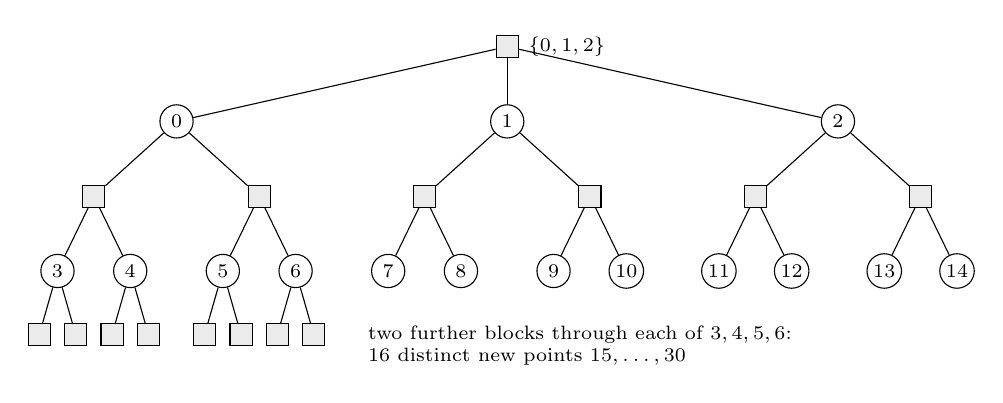
\begin{tikzpicture}[
  pt/.style={circle,draw,inner sep=1.2pt,minimum size=12pt,font=\scriptsize},
  bl/.style={rectangle,draw,fill=black!8,inner sep=1.5pt,minimum size=8pt},
  x=0.42cm,y=0.95cm]
  \node[bl] (r) at (0,4) {};
  \node[font=\scriptsize,right] at (r.east) {$\{0,1,2\}$};
  \foreach \p/\x in {0/-10,1/0,2/10} \node[pt] (p\p) at (\x,3) {\p};
  \foreach \p in {0,1,2} \draw (r)--(p\p);
  % second level blocks and points 3..14
  \foreach \a/\b/\c/\x in {0/3/4/-12.5,0/5/6/-7.5,1/7/8/-2.5,1/9/10/2.5,2/11/12/7.5,2/13/14/12.5}{
    \node[bl] (b\b) at (\x,2) {};
    \draw (p\a)--(b\b);
    \node[pt] (p\b) at (\x-1.1,1) {\b};
    \node[pt] (p\c) at (\x+1.1,1) {\c};
    \draw (b\b)--(p\b); \draw (b\b)--(p\c);
  }
  % third level from 3..6
  \foreach \p/\x in {3/-13.6,4/-11.4,5/-8.6,6/-6.4}{
    \node[bl] (c\p a) at (\x-0.55,0.15) {};
    \node[bl] (c\p b) at (\x+0.55,0.15) {};
    \draw (p\p)--(c\p a); \draw (p\p)--(c\p b);
  }
  \node[font=\scriptsize,align=left,anchor=west] at (-4.5,0.0) {two further blocks through each of $3,4,5,6$:\\ $16$ distinct new points $15,\dots,30$};
\end{tikzpicture}
\caption{The root of Branch B (\cref{lem:moore-root}): $15$ blocks on $31$
points in the Levi graph. Squares are blocks, circles are points.}
\label{fig:root}
\end{figure}

%======================================================================
\section{Certificates and checking}\label{sec:certs}

For every proposal that passes the degree and pair tests, the search program
writes one record to a stream: either \emph{expand}, or a rejection with the
indices of the blocks of a witness from \cref{lem:incremental} ($2$ blocks for
a $6$-cycle, $3$ for an $8$-cycle, $7$ for a $16$-cycle, plus the pair of
points of the candidate at which the $16$-cycle is closed). The cycle searches in
the generator only produce witnesses.

The \emph{checker} rebuilds the root and replays the schedule of
\cref{sec:search} from the stream. It recomputes every structural rejection
itself, and for every cycle record it checks that the named blocks are distinct
and already present, that consecutive blocks meet in exactly one point, that the
first and last block contain the two prescribed points of the candidate, and
that all points of the cycle are distinct. It never searches for a cycle. It
fails if the stream reaches a completed configuration, if a record is malformed,
if bytes are left over, or if its counters differ from those of the generator.

Branch~B is run as a single stream for each cap, written to a file and checked
by a separate program (\code{girth10\_search} and \code{girth10\_verify}).
Branch~A at caps $40$--$42$ is too large for one stream ($134$\,GB at cap $42$),
so the program \code{triangle\_search} splits the tree into subtrees that
worker threads take from a shared queue. Each subtree, and each splitting step,
has its own stream, which the checker class replays from the subtree root
before the work is counted; for a splitting step it also requires the list of
child subtrees to be identical. Every subtree therefore has a checked parent,
and the counters add up to those of the single-threaded program.

%======================================================================
\section{Results}\label{sec:results}

\Cref{tab:branchA,tab:branchB} list the counters. All runs end with zero
completions, and all streams are accepted by the checkers. Times are wall-clock
times on a $16$-core AMD Ryzen~9 7950X3D.

\begin{table}[ht]
\centering
\small
\caption{Branch A (configurations with a Berge triangle), by cap $v$ and root
orbit. ``Structural'' counts degree and pair rejections; $C_8$ and $C_{16}$
count rejections with a witness cycle. Caps $29$ and $34$ reproduce~\cite{Tranquilli2026,Zhuge2026}.}
\label{tab:branchA}
\begin{tabular}{@{}rcrrrrr@{}}
\toprule
$v$ ($n\le 2v$) & orbit & states & proposals & structural & $C_8$ & $C_{16}$\\
\midrule
29 (58) & 1 & 1{,}405 & 106{,}964 & 7{,}184 & 63{,}526 & 34{,}850\\
        & 2 & 20{,}088 & 1{,}655{,}404 & 113{,}012 & 1{,}208{,}473 & 313{,}832\\
34 (68) & 1 & 23{,}143 & 2{,}972{,}750 & 180{,}011 & 1{,}424{,}785 & 1{,}344{,}812\\
        & 2 & 202{,}602 & 25{,}227{,}209 & 1{,}432{,}521 & 15{,}207{,}779 & 8{,}384{,}308\\
40 (80) & 1 & 1{,}763{,}196 & 354{,}095{,}363 & 18{,}070{,}520 & 148{,}081{,}803 & 186{,}179{,}845\\
        & 2 & 12{,}393{,}295 & 2{,}606{,}532{,}806 & 135{,}470{,}813 & 1{,}036{,}826{,}697 & 1{,}421{,}842{,}002\\
41 (82) & 1 & 3{,}111{,}947 & 618{,}690{,}795 & 31{,}187{,}384 & 281{,}123{,}347 & 303{,}268{,}118\\
        & 2 & 30{,}997{,}584 & 7{,}353{,}663{,}962 & 373{,}859{,}991 & 2{,}860{,}026{,}335 & 4{,}088{,}780{,}053\\
42 (84) & 1 & 5{,}517{,}089 & 1{,}141{,}100{,}929 & 56{,}503{,}556 & 567{,}886{,}245 & 511{,}194{,}040\\
        & 2 & 73{,}104{,}843 & 19{,}186{,}516{,}084 & 936{,}237{,}621 & 7{,}358{,}733{,}813 & 10{,}818{,}439{,}808\\
\bottomrule
\end{tabular}
\end{table}

The run at cap $42$ took $561$\,s with $16$ threads and wrote and checked
$134$\,GB of witness streams in memory.

\begin{table}[ht]
\centering
\small
\caption{Branch B (Levi graph of girth at least $10$), by cap $v$.}
\label{tab:branchB}
\begin{tabular}{@{}rrrrrrr@{}}
\toprule
$v$ ($n\le 2v$) & states & proposals & structural & $C_6$ & $C_8$ & $C_{16}$\\
\midrule
35 (70) & 28{,}995 & 6{,}416{,}316 & 334{,}752 & 1{,}013{,}910 & 4{,}217{,}540 & 821{,}120\\
36 (72) & 41{,}571 & 8{,}044{,}454 & 395{,}768 & 1{,}150{,}772 & 5{,}301{,}400 & 1{,}154{,}944\\
37 (74) & 55{,}684 & 8{,}406{,}847 & 407{,}992 & 1{,}181{,}052 & 5{,}521{,}416 & 1{,}240{,}704\\
38 (76) & 69{,}092 & 11{,}408{,}831 & 544{,}920 & 2{,}255{,}036 & 7{,}044{,}104 & 1{,}495{,}680\\
39 (78) & 83{,}749 & 16{,}916{,}906 & 768{,}230 & 4{,}114{,}728 & 9{,}884{,}728 & 2{,}065{,}472\\
40 (80) & 99{,}477 & 19{,}929{,}254 & 875{,}102 & 5{,}053{,}904 & 11{,}441{,}060 & 2{,}459{,}712\\
41 (82) & 122{,}678 & 21{,}779{,}839 & 960{,}350 & 5{,}771{,}896 & 12{,}326{,}772 & 2{,}598{,}144\\
42 (84) & 151{,}270 & 30{,}152{,}223 & 1{,}310{,}846 & 7{,}802{,}760 & 14{,}160{,}948 & 6{,}726{,}400\\
43 (86) & 430{,}471 & 66{,}385{,}632 & 3{,}039{,}214 & 16{,}168{,}760 & 23{,}969{,}780 & 22{,}777{,}408\\
44 (88) & 1{,}192{,}135 & 259{,}856{,}800 & 11{,}307{,}910 & 84{,}761{,}220 & 72{,}703{,}376 & 89{,}892{,}160\\
\bottomrule
\end{tabular}
\end{table}

\begin{proof}[Proof of \cref{thm:main}]
Suppose $G$ is a cubic bipartite graph on at most $84$ vertices without cycles of
length $4$, $8$ and $16$. A connected component of $G$ has the same properties,
so we may assume $G$ connected; let $\mathcal T$ be its configuration, with
$v\le 42$ points. It is linear and has no Berge quadrilateral or octagon. If $G$
has a $6$-cycle, \cref{lem:triangle,prop:coverage} show that Branch~A with cap
$42$ reaches $\mathcal T$ as a completion. Otherwise, by \cref{lem:dichotomy},
$G$ has girth at least $10$, and \cref{lem:moore-root,prop:coverage} show that
Branch~B with cap $42$ reaches it. Both searches have no completion.
\end{proof}

\begin{proof}[Proof of \cref{thm:girth10}]
The same argument with Branch~B alone and cap $44$; a graph of girth at least
$10$ has no $4$-, $6$- or $8$-cycle, so only the $16$-cycle can be missing.
\end{proof}

%======================================================================
\section{Validation}\label{sec:validation}

The checkers establish that every rejection is justified. The remaining risk is
an error in the enumeration, that is, in the implementation of
\cref{prop:coverage}. We test it in four ways.

\begin{enumerate}[leftmargin=2em,label=(\alph*)]
\item \emph{Tranquilli's program.} Branch~A uses the schedule of Tranquilli's
  \code{triangle\_root\_\allowbreak universal\_\allowbreak search.cpp} (commit \code{67adc92d}, whose
  SHA-256 we checked against the published manifest). We compiled that program,
  unchanged, for the caps $20,22,24,26,29,34,35,\dots,42$. For every cap and
  orbit, all six counters agree with \cref{tab:branchA}. Tranquilli's program
  is single-threaded and does not share the subtree splitting.
\item \emph{An independent implementation.} The file
  \code{independent\_check.py} implements both schedules from their description
  in \cref{sec:search}, in Python, without any code in common with the C++
  programs. It decides each cycle test by asking for a simple path of the
  required length in the Levi graph (\cref{lem:incremental}) instead of
  enumerating Berge cycles. For Branch~A at caps $20$--$26$ and Branch~B at
  caps $31$--$33$ all counters agree with the C++ programs.
\item \emph{Coverage on the cages.} The three
  $(3,10)$-cages~\cite{OKeefeWong1980,Wong1983} have girth $10$ and $70$ vertices. For each cage, each colour class taken as
  points and each of the $35$ root blocks, \code{independent\_check.py} labels
  the cage as in \cref{lem:moore-root,prop:coverage} and follows it through the
  Branch~B schedule with the $16$-cycle test switched off. All $210$ replays are
  accepted at every step and end in a completion. With the $16$-cycle test on,
  each replay is rejected by a $16$-cycle, in agreement with
  \cref{thm:girth10}.
\item \emph{Small orders.} At caps up to $13$, Tranquilli compared the
  configurations generated by his program, with the cycle tests switched off,
  against nauty's \code{genbg} and the census of Betten, Brinkmann and
  Pisanski~\cite[§4]{Tranquilli2026}. This validates the schedule itself, which
  both of our searches use.
\end{enumerate}

%======================================================================
\section{Formalization}\label{sec:lean}

The file \code{lean/ErdosGyarfas/CubicBipartite.lean} of the repository proves,
in Lean~4~\cite{Lean4} without external libraries and with only Lean's standard
axioms:
\begin{itemize}[leftmargin=1.5em]
\item \lean{bipartite\_cycle\_even} and \lean{bipartite\_no\_c4\_c8\_dichotomy}:
  \cref{lem:dichotomy};
\item for the incidence graph of a $3$-uniform, $3$-regular linear configuration:
  it is bipartite and has no $4$-cycle (\lean{toGraph\_isBipartite},
  \lean{toGraph\_no\_C4});
\item \lean{alternating\_cycle\_sound}: $m\ge 2$ distinct points and $m$
  distinct blocks with $p_i,p_{i+1}\in B_i$ give a $2m$-cycle; the special cases
  $m=3,4,8$ (\lean{check\_c6\_witness\_sound}, \lean{check\_c8\_witness\_sound},
  \lean{check\_c16\_witness\_sound}) are exactly the conditions tested by the
  checkers;
\item \lean{c6\_two\_orbit\_dichotomy}: the case analysis of \cref{lem:triangle};
\item \lean{girth10\_moore\_tree\_62}: a cubic graph of girth at least $10$ has
  at least $62$ vertices, the vertex count underlying \cref{lem:moore-root}.
\end{itemize}
The formalization does not cover \cref{prop:coverage}, the root labelling of
\cref{lem:moore-root}, or the correctness of the C++ programs. For this reason
we regard \cref{thm:main} as a computer-assisted result, verified by the
cross-checks of \cref{sec:validation}, and not as a formally verified one.

%======================================================================
\section{Reproducibility}\label{sec:repro}

Everything is in the folder \code{results/cubic-bipartite-power-of-two-cycles} of
\url{https://github.com/hipotures/conjectures}. The programs in \code{src/} are
adapted from Tranquilli's code and are distributed under the MIT License; the
rest of the repository is in the public domain (CC0). The script
\code{reproduce.py} compiles the programs, runs Branch~A at caps $29$, $34$, $35$,
$40$, $41$, $42$ and Branch~B at caps $35$--$44$, checks every witness stream,
and compares all counters with \code{data/expected\_counts.json}. A full run
takes about $15$ minutes on $16$ cores and needs no disk space beyond the largest
Branch~B stream ($1.3$\,GB). The file \code{data/upstream\_crosscheck.json}
records the output of Tranquilli's program, including its transcript hashes,
and \code{independent\_check.py} runs checks (b) and (c) of
\cref{sec:validation} in about half a minute.

\section*{Use of AI tools}
This work was carried out with substantial assistance from AI systems, mainly
Gemini~4~Neon (Google) and Claude Opus~5.5 (Anthropic), used through the
Antigravity and Claude Code environments. They were used to write and run the
search and checking programs, the Lean development and the independent checks,
and to draft the text. AI systems are not authors of this paper. The author
takes responsibility for the content and for the attribution of prior work.

\section*{Acknowledgements}
The triangle-rooted search, its certificate format and the coverage argument
are due to Julius Tranquilli, whose code is openly licensed; this work extends
it. We also thank Yihan Zhuge for the open artifact of the $70$-vertex bound.

\begin{thebibliography}{99}

\bibitem{BettenBrinkmannPisanski2000}
A.~Betten, G.~Brinkmann and T.~Pisanski, \emph{Counting symmetric
configurations $v_3$}, Discrete Appl. Math. \textbf{99} (2000), 331--338.

\bibitem{DucoffeDumitru2026}
G.~Ducoffe and B.~Dumitru, \emph{Towards a more structured search for
Erdős--Gyárfás counter-examples}, arXiv:2609.28594, 2026.

\bibitem{Erdos1997}
P.~Erdős, \emph{Some old and new problems in various branches of combinatorics},
Discrete Math. \textbf{165/166} (1997), 227--231.

\bibitem{Exoo2014}
G.~Exoo, \emph{Three graphs and the Erdős--Gyárfás conjecture},
arXiv:1403.5636, 2014.

\bibitem{Lean4}
L.~de Moura and S.~Ullrich, \emph{The Lean 4 theorem prover and programming
language}, in: Automated Deduction -- CADE 28, Lecture Notes in Comput. Sci.
\textbf{12699}, Springer, 2021, 625--635.

\bibitem{Marszalek2026}
A.~Marszałek, \emph{Small graphs without cycles of length a power of two: new
bounds with kernel-checked proofs}, preprint, 2026,
\url{https://doi.org/10.5281/zenodo.24588313}.

\bibitem{OKeefeWong1980}
M.~O'Keefe and P.~K.~Wong, \emph{A smallest graph of girth 10 and valency 3},
J. Combin. Theory Ser. B \textbf{29} (1980), 91--105.

\bibitem{Ripatti2017}
A.~V.~Ripatti, \emph{Faster approach for exhaustive search over graphs with
certain properties}, abstract, BAIKAL 2017 conference, 2017.

\bibitem{Tranquilli2026}
J.~Tranquilli, \emph{A 60-vertex lower bound for cubic bipartite
counterexamples to the Erdős--Gyárfás conjecture}, arXiv:2608.02675, 2026.
Code: \url{https://github.com/floor-licker/erdos-gyarfas-cubic-bipartite}.

\bibitem{Wong1983}
P.~K.~Wong, \emph{On the smallest graphs of girth 10 and valency 3}, Discrete
Math. \textbf{43} (1983), 119--124, \url{https://doi.org/10.1016/0012-365X(83)90029-8}.

\bibitem{Zhuge2026}
Y.~Zhuge, \emph{A 70-vertex lower bound for cubic bipartite counterexamples to
the Erdős--Gyárfás conjecture}, preprint and artifact, Zenodo, 2026,
\url{https://doi.org/10.5281/zenodo.21981786}.

\end{thebibliography}

\end{document}
